\documentclass[a4paper,10pt,ngerman]{scrartcl}
\usepackage{babel}
\usepackage[T1]{fontenc}
\usepackage[utf8x]{inputenc}
\usepackage[a4paper,margin=2.5cm,footskip=0.5cm]{geometry}

% Die nächsten drei Felder bitte anpassen:
\newcommand{\Aufgabe}{Aufgabe 3: Lieferkette} % Aufgabennummer und Aufgabennamen angeben
\newcommand{\TeilnahmeId}{79418}                  % Teilnahme-ID angeben
\newcommand{\Name}{Fabian Schwarz}             % Name des Bearbeiter / der Bearbeiterin dieser Aufgabe angeben


% Kopf- und Fußzeilen
\usepackage{scrlayer-scrpage, lastpage}
\setkomafont{pageheadfoot}{\large\textrm}
\lohead{\Aufgabe}
\cohead{\Name}
\rohead{Teilnahme-ID: \TeilnahmeId}
\cfoot*{\thepage{}/\pageref{LastPage}}

% Position des Titels
\usepackage{titling}
\setlength{\droptitle}{-1.0cm}

% Für mathematische Befehle und Symbole
\usepackage{amsmath}
\usepackage{amssymb}

% Für Bilder
\usepackage{graphicx}

% Für Algorithmen
\usepackage{algpseudocode}

% Für Quelltext
\usepackage{listings, listings-rust}
\usepackage{color}
\definecolor{mygreen}{rgb}{0,0.6,0}
\definecolor{mygray}{rgb}{0.5,0.5,0.5}
\definecolor{mymauve}{rgb}{0.58,0,0.82}
\lstset{
    keywordstyle=\color{blue},commentstyle=\color{mygreen},
    stringstyle=\color{mymauve},rulecolor=\color{black},
    basicstyle=\footnotesize\ttfamily,numberstyle=\tiny\color{mygray},
    captionpos=b, % sets the caption-position to bottom
    keepspaces=true, % keeps spaces in text
    numbers=left, numbersep=5pt, showspaces=false,showstringspaces=true,
    showtabs=false, stepnumber=2, tabsize=2, title=\lstname
}
\lstdefinelanguage{JavaScript}{ % JavaScript ist als einzige Sprache noch nicht vordefiniert
    keywords={break, case, catch, continue, debugger, default, delete, do, else, finally, for, function, if, in, instanceof, new, return, switch, this, throw, try, typeof, var, void, while, with},
    morecomment=[l]{//},
    morecomment=[s]{/*}{*/},
    morestring=[b]',
    morestring=[b]",
    sensitive=true
}

% Diese beiden Pakete müssen zuletzt geladen werden
\usepackage{amsopn}
\usepackage{amstext}
\usepackage{hyperref}
\usepackage{cleveref}

% Daten für die Titelseite
\title{\textbf{\Huge\Aufgabe}}
\author{\LARGE Teilnahme-ID: \LARGE \TeilnahmeId \\\\
\LARGE Bearbeiter/-in dieser Aufgabe: \\
\LARGE \Name\\\\}
\date{\LARGE\today}

\lstdefinestyle{plain}{
    language={},
    keywordstyle=\color{black},
    commentstyle=\color{black},
    stringstyle=\color{black},
    numbers=none,
    italicconsole=false
}

\lstset{frame=tb,
    language=Rust,
    aboveskip=3mm,
    belowskip=1mm,
    showstringspaces=false,
    columns=flexible,
    basicstyle={\small\ttfamily},
    numbers=none,
    numberstyle=\tiny\color{gray},
    keywordstyle=\color{blue},
    commentstyle=\color{dkgreen},
    stringstyle=\color{mauve},
    breaklines=true,
    breakatwhitespace=true,
    tabsize=3
}

\begin{document}

    \maketitle
    \tableofcontents

    \vspace{0.5cm}


    \section{Lösungsidee}
    Zu Beginn sollen die Werke und ihre Verbindungen als gewichteter, ungerichteter Graph dargestellt werden, wobei das
    Gewicht jeder Kante die benötigte Fahrzeit für diese Straße darstellt. Hierfür gruppiert man die Werke in
    funktionale Gruppen $G_1, \dots, G_n$, mit $n$ als Anzahl der benötigten Arbeitsschritte, wobei $G_k$ alle
    Knoten (Werke) beinhaltet, die den Arbeitsschritt $k$ erfüllen können. Für jedes Paar von Werken $(u, v)$ wird nun
    die kürzeste Fahrtzeit $d(u, v)$ bestimmt und gespeichert.
    Diese $G_k$ stellen nun die $k$ Schichten eines Schichtengraphen dar.

    Man definiert $S(u)$ als den optimalen Restweg vom Werk $u$ zum Ziel $z$:
    \[
        S(u) =
        \begin{cases}
            d(u, z) & \text{für } u \in G_n \\
            \min_{w \in G_{k+1}} \{ d(u, w) + S(w) \} & \text{für } u \in G_k : k < n
        \end{cases}
    \]

    und $R(v)$ als ``Streikkosten'', also die übrige Zeit bis zum Ziel $z$, wenn die Fahrerin gerade vor dem streikenden
    Werk $v$ steht:
    \[
        R(v) = \min_{u \in G_k \setminus \{v\}} \left( \underbrace{d(v, u)}_{\text{Fahrt zum Ersatz}} + \underbrace{S(u)}_{\text{Restweg ab dort}} \right)
    \]

    Hierbei sind zwei Sonderfälle zu beachten:
    \begin{itemize}
        \item Wenn $|G_k| = 1$ ist $R(v) = \infty$ und somit kann der Weg nicht streik-sicher sein.
        \item $R(z) = 0$.
    \end{itemize}

    Für jeden Arbeitsschritt $k$ betrachtet man nun die frühestmögliche Ankunftszeit unter Betrachtung eines
    möglichen Streiks $A(v)$ an jedem Werk $v \in G_k$. Für den Start $s$ ist $A(s) = 0$. Um diese zu bestimmen, werden
    alle Werke $u \in G_{k-1}$ betrachtet:
    \[
        A(v) = \min \{ A(u) + d(u, v) \mid u \in G_{k-1} \wedge A(u) + d(u, v) + R(v) \leq T \}
    \]
    wobei $T$ die maximal erlaubte Bearbeitungszeit ist. Damit ist garantiert, dass:
    \begin{enumerate}
        \item Alle vorherigen Werke bereits sicher (i.e.\ in $T$ erreichbar) sind, da $A(u)$ schon geprüft wurde,
        \item wenn genau bei $v$ gestreikt wird, der Weg dennoch sicher ist und
        \item der schnellste Pfad ausgewählt wird.
    \end{enumerate}

    Sobald man bei $z$ ankommt, wird geprüft, ob $A(z) \leq T$. Falls ja, existiert ein Pfad, der jeden möglichen Streik
    in $T$ umgehen kann.

    Um die Pläne auszugeben, werden während der Berechnung Pointer auf die jeweiligen Optima gespeichert:
    \begin{itemize}
        \item Die Normalroute wird durch das Speichern des jeweils optimalen Vorgängers $u \in G_{k-1}$ während der Berechnung von $A(v)$ ermittelt. Sobald das Ziel $z$ erreicht ist, lässt sich die gesamte Strecke durch einfaches rückwärtiges Verfolgen dieser Pointer bis zum Startpunkt $s$ rekonstruieren.
        \item Für jedes Werk $v_i$, das Teil dieser Normalroute ist, wird zusätzlich ein individueller Alternativplan bereitgestellt. Sollte vor Ort ein Streik an $v_i$ festgestellt werden, steuert die Fahrerin zunächst das Ersatzwerk $u \in G_k \setminus \{v_i\}$ an, welches bei der Berechnung von $R(v_i)$ das zeitliche Minimum geliefert hat.
        \item Von diesem Ersatzwerk $u$ aus folgt die weitere Fahrt einer Kette von Idealschritten bis zum Ziel $z$. Diese Kette setzt sich aus den jeweiligen Nachfolgern $w \in G_{k+1}$ zusammen, die bereits während der Rückwärtsrechnung von $S(u)$ als lokales Minimum, also als der jeweils nächste optimale Schritt, identifiziert und für jedes Werk hinterlegt wurden.
    \end{itemize}

    Wie sich in der \hyperref[sec:laufzeit]{Laufzeitberechnung} herausstellt, ist dieser Ansatz auch für das größte
    Beispiel (Nummer 10 mit $N = 3932$ und $M = 26040$) in wenigen Sekunden lösbar, weshalb keine weiteren
    Lösungsansätze betrachten wurden.

    \section{Umsetzung}
    \subsection{Datenstrukturen}
    Die Straßenkarte wird als ungerichteter Graph mit der Fahrtzeit als Kantengewicht eingelesen.
    Bereits jetzt werden die Werke nach ihrem Arbeitsschritt in die Gruppen $G_k$ gruppiert.

    Für jeden Interessepunkt, also den Startpunkt $S$ und alle Werke, wird ein Single-Source Shortest Path Dijkstra
    \footnote{Raman, R. (1997). Recent results on the single-source shortest paths problem.
    \textit{ACM SIGACT News}, \textit{28}(2), 81–87. \url{https://doi.org/10.1145/261342.261352}}
    ausgeführt. Dieser ist in der verwendeten \textit{petgraph} Bibliothek bereits optimal (unter Verwendung einer
    priority-queue) implementiert. Die Ergebnisse werden in einer geschachtelten \texttt{HashMap all\_dists} gespeichert,
    um in $O(1)$ die Distanz zwischen zwei beliebigen Werken $u, v$ als \texttt{all\_dists[u][v]} abfragen zu können.

    \subsection{Restwege und Streikkosten}
    Nun wird jeder Arbeitsschritt $k$ von $n$ bis $1$ rückwärts durchlaufen. Für jedes Werk wird der optimale
    Restweg zum Ziel berechnet und gespeichert. Gleichzeitig wird für jedes Werk $v$ eine \texttt{backup\_node}, also
    das beste Ausweichwerk im Fall eines Streiks, bestimmt, und daraus die resultierenden Streikkosten $R(v)$.

    \subsection{Bestimmung der sicheren Route}
    Als nächstes werden in einem Vorwärtsdurchlauf für jedes Werk $v$ in Schicht $k$ alle Vorgängerknoten $u$ aus
    Schicht $k - 1$ geprüft. Ein Übergang wird nur gespeichert, wenn er sicher ist, also $A(u) + d(u,v) + R(v) \leq T$
    erfüllt ist. Dies garantiert, dass bei einem Streik an egal welchem Werk $v$ die Frist nie überschritten wird.
    Ist dies nicht erfüllbar, scheitert der Algorithmus und es gibt keine vollkommen sichere Route.

    \subsection{Rekonstruktion und Ausweichrouten}
    Nachdem die sichere Erreichbarkeit des Ziels überprüft wurde, also $A(z) \leq T$, werden die Pfade zurückverfolgt.
    Ausgehend von einer vorhin gespeicherten Map \texttt{prev\_secure} wird schrittweise für jedes Werk der optimale
    Vorgänger bestimmt, bis der Startpunkt erreicht ist.

    Für jedes Werk $v$ der Hauptroute wird ein individueller Plan erstellt. Hierbei wird der A*-Algorithmus\footnote{
    Die Heuristik ist hier 0, was heißt, dass eigentlich einfach nur der Dijkstra-Algorithmus angewandt wird.
        Unterschied bei diesem Methodenaufruf ist, dass so der konkrete Pfad zurückgegeben wird, und nicht nur dessen
        Länge; das ist somit bibliotheksbedingt.
    }
    aus \texttt{petgraph} benutzt,der den konkreten Pfad von Werk $v$ zur vorhin hinterlegten \texttt{backup\_node}
    bestimmt. Ab hier wird die Route durch die Kette der vorhin hinterlegten nächstbesten Knoten berechnet.

    Die Ergebnisse werden folgend ausgegeben und visualisiert.

    \section{Laufzeit}\label{sec:laufzeit}
    Um die kürzesten Wege zwischen allen Paaren von Werken zu berechnen wird der Dijkstra-Algorithmus verwendet, der
    N mal ausgeführt werden muss, für $N$ Werke, $M$ Straßen und $n$ Arbeitsschritte. Der Graph scheint recht dünn, mit
    nur durchschnittlich 7 Straßen pro Werk im größten Beispiel (Beispiel 10), weshalb unter der verwendeten
    Implementierung von einer Laufzeitkomplexität von $O(N(M + N \log N))$ ausgegangen werden kann.
    \footnote{\label{fn:dijkstra}Fredman, M. L., \& Tarjan, R. E. (1987).
    Fibonacci heaps and their uses in improved network optimization algorithms.
    \textit{Journal of the ACM}, \textit{34}(3), 596–615. \url{https://doi.org/10.1145/28869.28874}}

    Bei der Berechnung von $S(u)$ werden für jedes Werk in $G_k$ alle Werke in $G_{k+1}$ betrachtet. Die Anzahl an
    Vergleichen ist somit durch die Anzahl der Werk-Paare begrenzt, womit $S(u) \in O(N^2)$.
    Aus dem selben Grund ist $R(v) \in O(N^2)$ für den Worst-Case, dass alle Werke in die selbe Gruppe $G_k$ fallen.

    Analog zu der Bestimmung der Komplexität von $S(u)$ ist auch $A(v) \in O(N^2)$.

    Die Gesamtlaufzeit bestimmt sich also auf $O(NM + N^2 \log N)$.

    Für das größte Beispiel mit $N = 3932$ und $M = 26040$ lässt sich die Belastung also auf circa $300 * 10^6$
    Operationen für den Dijkstra-Algorithmus und $16 * 10^6$ Operationen für die $S$, $R$ und $A$ Tabellen bestimmen,
    womit sich die Gesamtlaufzeit selbst ohne Multithreading im Bereich weniger Sekunden halten sollte
    \footnote{8 x 11th Gen Intel(R) Core(TM) i5-1145G7 @ 2.60GHz}.


    \section{Werkzeuge}
    Der Code wurde vollständig in Rust 1.93.1 (01f6ddf75 2026-02-11) geschrieben.\\
    Das \href{https://crates.io/crates/petgraph}{\texttt{petgraph} Crate}
    wurde für eine optimierte Implementierung von Graphen verwendet. Es verwaltet die Lifetimes von Knoten und Kanten
    intern, was einigen Boilerplate-Code erspart. Die mitgelieferte Implementierung des Dijkstra-Algorithmus folgt dem
    min-heap priority queue Ansatz aus Fredman \& Tarjan (1987)\footnote{Siehe \cref{fn:dijkstra}.}. Ebenfalls wird die
    Implementierung des A*-Algorithmus mit der Heuristik $0$ verwendet, um am Ende das Backtracking auszuführen, da der
    eingebaute Dijkstra-Algorithmus die Pfade nicht zurückgibt.\\

    \section{Beispiele}
    \subsection{Beispiel 00}
    \begin{lstlisting}[style=plain]
MOEGLICH
15

9
S [3 1] [5 2] T
11
3 [2 1] 3 [5 2] T
15
5 T [4 2] T
    \end{lstlisting}

    \noindent
    \begin{minipage}[t]{0.5\textwidth}
        \vspace{0pt}
        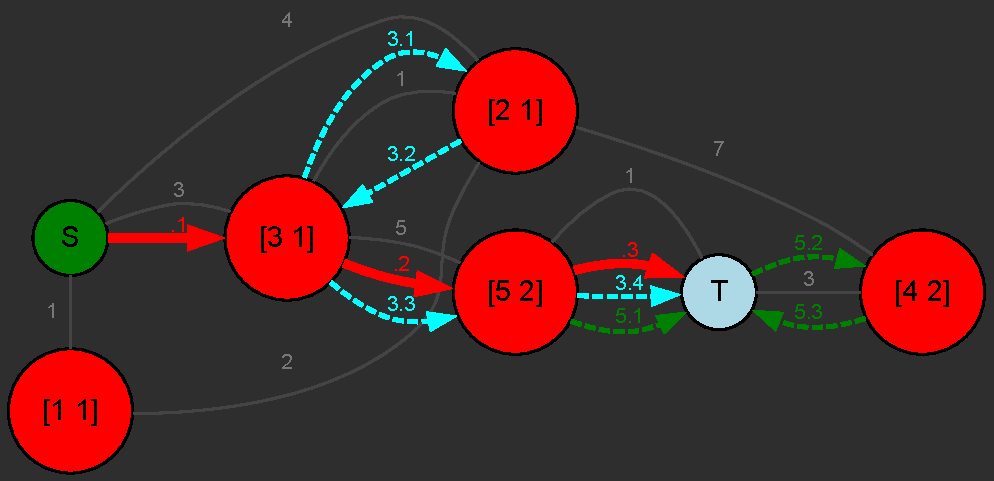
\includegraphics[width=\textwidth]{graphviz_00}
    \end{minipage}
    \hfill
    \begin{minipage}[t]{0.45\textwidth}
        \vspace{0pt}
        Die grauen Linien stellen hier die Straßen mit entsprechenden Gewichten (Fahrtzeiten) dar.
        Die Pfeile .1, .2, \dots zeigen den Standardpfad. Die Pfeile 3.1, 3.2, \dots zeigen den Ersatzpfad, für den Fall
        dass Werk 3 bestreikt wird, und so weiter. Werke sind hier als [N, K] dargestellt, wobei N die Nummer des Werks
        und K der dort machbare Verarbeitungsschritt ist.

        Diese Pfade sind offensichtlich optimal.
    \end{minipage}

    \subsection{Beispiel 01}
    \begin{lstlisting}[style=plain]
MOEGLICH
40

26
S [1 1] [4 2] [7 3] T
40
1 S [2 1] S 1 [4 2] [7 3] T
37
4 [5 2] [8 3] T
38
7 T [6 3] T
    \end{lstlisting}

    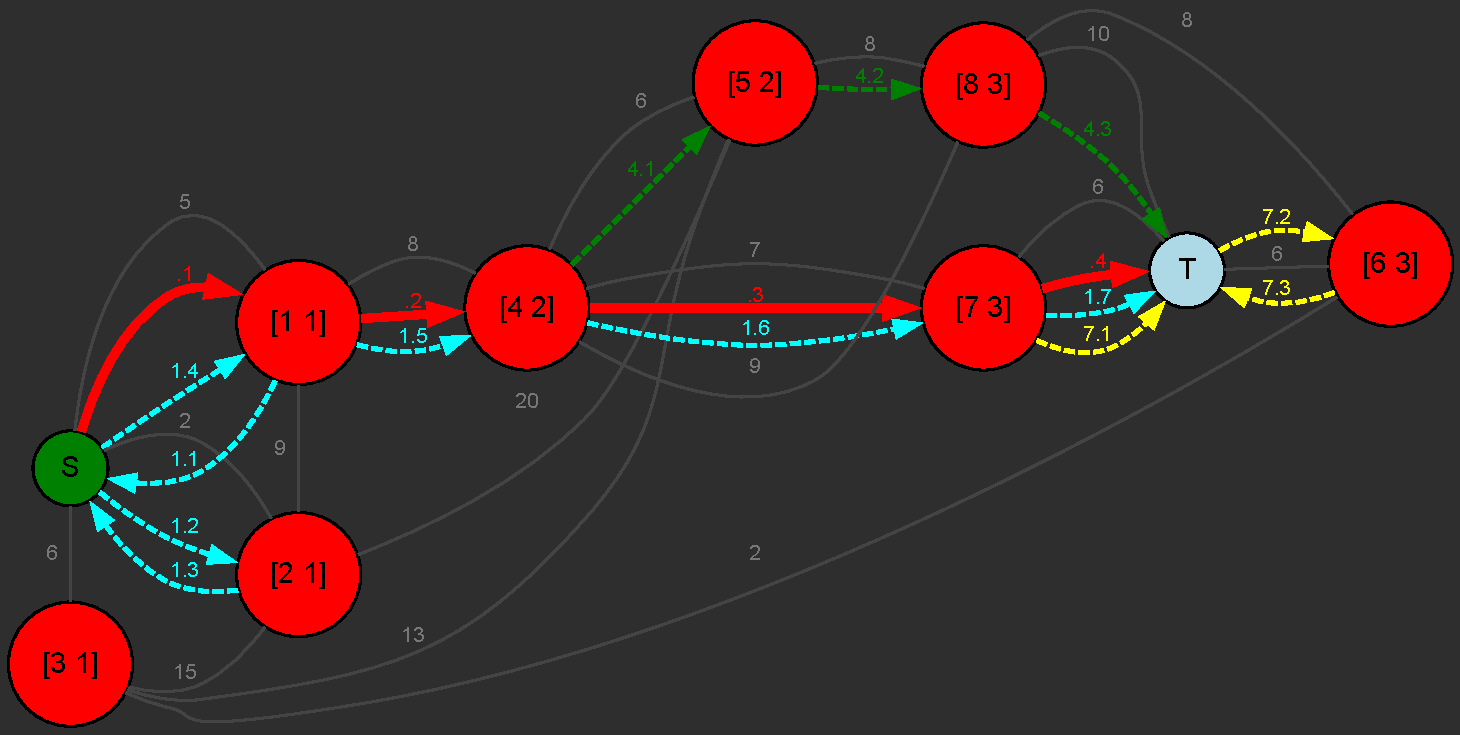
\includegraphics[width=\textwidth]{graphviz_01}
    Auch diese Pfade scheinen optimal.

    \subsection{Beispiel 02}
    \begin{lstlisting}[style=plain]
MOEGLICH
188

122
S [1 1] [2 2] [4 3] [10 4] [7 5] T
138
1 6 [5 1] [3 2] [4 3] 2 13 7 [10 4] [7 5] 13 2 S 1 T
157
2 13 7 5 [3 2] [4 3] 2 13 7 [10 4] [7 5] 13 2 S 1 T
188
4 3 5 6 12 [11 3] 9 8 [10 4] [7 5] 13 2 S 1 T
174
10 7 5 [6 4] 5 [7 5] 13 2 S 1 T
122
7 [13 5] 2 S 1 T
    \end{lstlisting}

    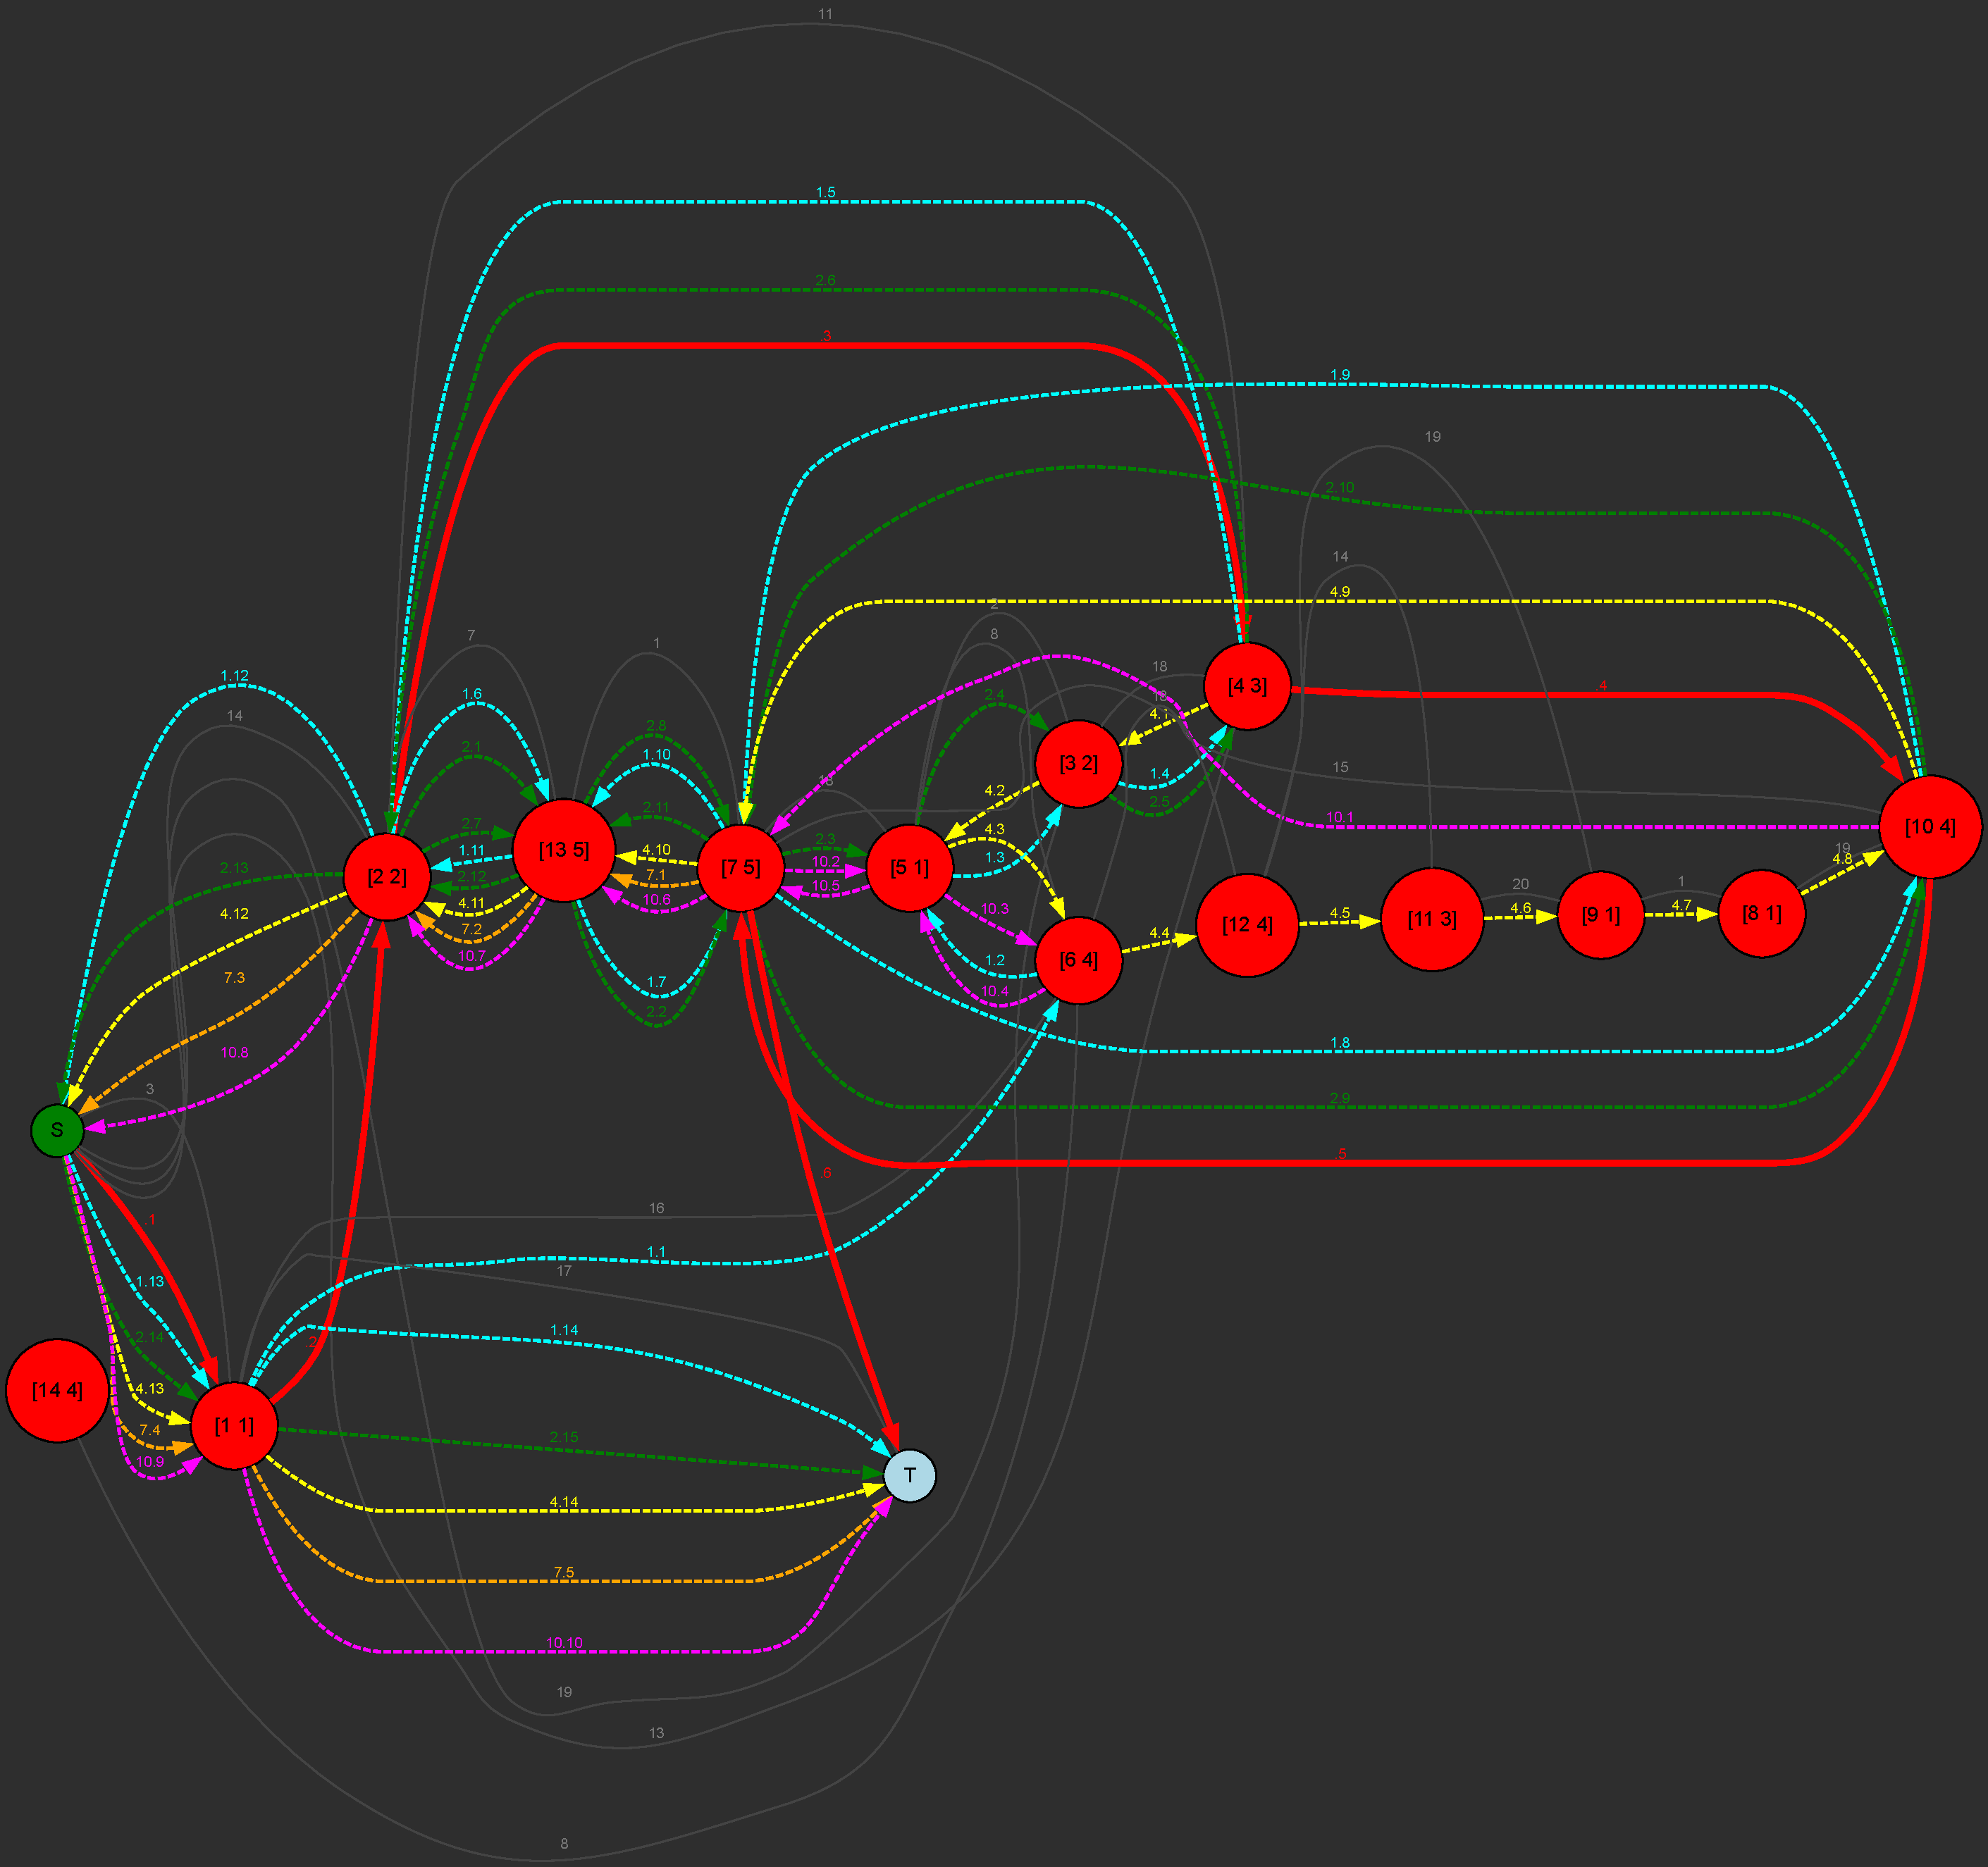
\includegraphics[width=\textwidth]{graphviz_02}

    Hier ist es schwierig zu erkennen, ob tatsächlich optimale Pfade gewählt worden sind. Die wiederholte Verwendung
    bestimmter Teilpfade auf unterschiedlichen Routen lässt dies jedoch vermuten; beispielsweise verwenden die
    Ersatzrouten für Werke 1, 2, 4 und 10 alle den Weg zu T über S, anstatt über Werk 7 wie der Standardpfad.

    \subsection{Beispiel 03}
    \begin{lstlisting}[style=plain]
UNMOEGLICH
    \end{lstlisting}

    \subsection{Beispiel 04}
    \begin{lstlisting}[style=plain]
MOEGLICH
264
[...]
    \end{lstlisting}

    \subsection{Beispiel 05}
    \begin{lstlisting}[style=plain]
MOEGLICH
930
[...]
    \end{lstlisting}

    \subsection{Beispiel 06}
    \begin{lstlisting}[style=plain]
UNMOEGLICH

    \end{lstlisting}

    \subsection{Beispiel 07}
    \begin{lstlisting}[style=plain]
MOEGLICH
675
[...]
    \end{lstlisting}

    \subsection{Beispiel 08}
    \begin{lstlisting}[style=plain]
MOEGLICH
1333
[...]
    \end{lstlisting}

    \subsection{Beispiel 09}
    \begin{lstlisting}[style=plain]
MOEGLICH
11
[...]
    \end{lstlisting}

    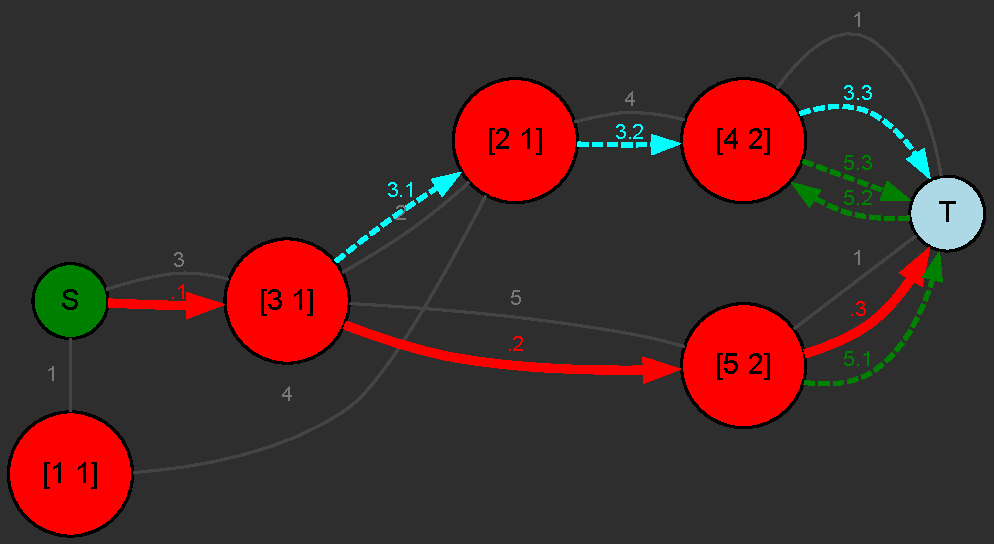
\includegraphics[width=\textwidth]{graphviz_09}

    Auch dieses Beispiel ist recht offensichtlich optimal.

    \subsection{Beispiel 10}
    \begin{lstlisting}[style=plain]
MOEGLICH
1462
[...]
    \end{lstlisting}

    \section{Quellcode}
    Auslassungen sind hier mit \texttt{/* [...] */} markiert.

    \begin{lstlisting}[style=colouredRust, label={lst:maincode}]
/* [...] */
fn solve() {
    /* [...] Einlesen der Datei und Initialisierung des Graphen [...] */

    // Für jeden relevanten Ort (Start und alle Werke) wird einmalig Dijkstra ausgeführt
    // Die Distanzen d(u, v) werden für O(1) Zugriff in einer Map gespeichert
    let mut all_dists = HashMap::new();
    for start in pois {
        let res = petgraph::algo::dijkstra(&graph, loc_to_idx[&start], None, |e| *e.weight());
        all_dists.insert(start, res.into_iter().map(|(i, d)| (graph[i].clone(), d)).collect());
    }

    // Rückwärts DP
    // s_val[u]: Optimaler Restweg von Werk u bis zum Ziel T
    // r_val[v]: Zeit bis Ziel, wenn Werk v bestreikt wird
    for step in (1..=data.count_steps).rev() {
        for &u in &data.grouped_factories[step as usize] {
            if step == data.count_steps {
                s_val.insert(u, all_dists[&u_loc][&LocationType::Goal]);
                next_best.insert(u, LocationType::Goal);
            } else {
                // Suche das Werk w im nächsten Schritt, das den Restweg minimiert
                /* [...] Minimum-Suche über alle w in G_{step+1} [...] */
                s_val.insert(u, min_dist);
                next_best.insert(u, best_w);
            }
        }

        // Berechnung des besten Ersatzwerks u in der selben Gruppe
        for &v in &data.grouped_factories[step as usize] {
            /* [...] Suche u in G_{step} \ {v}, das d(v, u) + s_val[u] minimiert [...] */
            r_val.insert(v, min_repair_dist);
            backup_node.insert(v, best_backup);
        }
    }

    // Vorwärts DP
    // a_val[v]: Früheste Ankunftszeit bei v, die garantieren kann, dass bei einem
    // anschließenden Streik von v das Ziel noch innerhalb von max_time erreicht wird
    a_val.insert(LocationType::Start, 0);
    for step in 1..=data.count_steps {
        for &v in &data.grouped_factories[step as usize] {
            // Prüfe alle potentiellen Vorgänger u aus der vorherigen Schicht
            for u_l in prev_layer {
                let d = all_dists[&u_l][&v_loc];
                if a_val[&u_l] + d + r_val[&v] <= data.max_time as i32 {
                    /* [...] Update a_val[v] und Speicherung des Vorgängers in prev_secure [...] */
                }
            }
        }
    }

    if final_a <= data.max_time as i32 {
        /* [...] Backtracking-Loop [...] */

        // Alternativrouten
        for node in &main_route {
            if let LocationType::Num(id) = node.loc {
                // Pfad zum Ersatzwerk mit Dijkstra (A* mit Heuristik 0)
                let (path_to_backup) = petgraph::algo::astar(&graph, /* [...] */);
                /* [...] Folgen der next_best Kette [...] */
            }
        }
    } else {
        /* [...] Unmöglich */
    }
}
    \end{lstlisting}

\end{document}
